% Created 2022-11-05 Sat 17:04
% Intended LaTeX compiler: pdflatex
\documentclass[10pt]{beamer}
\usepackage[utf8]{inputenc}
\usepackage[T1]{fontenc}
\usepackage{graphicx}
\usepackage{longtable}
\usepackage{wrapfig}
\usepackage{rotating}
\usepackage[normalem]{ulem}
\usepackage{amsmath}
\usepackage{amssymb}
\usepackage{capt-of}
\usepackage{hyperref}
\usepackage{minted}
\usepackage{xcolor}
\definecolor{LightGray}{gray}{0.95}
\usefonttheme{professionalfonts}
\setlength{\parskip}{5pt}
\newcommand{\footnoteframe}[1]{\footnote[frame]{#1}}
\addtobeamertemplate{footnote}{}{\vspace{2ex}}
\usepackage{tabularx}
\usepackage{booktabs}
\DefineVerbatimEnvironment{verbatim}{Verbatim}{fontsize=\scriptsize}
\usetheme{Berkeley}
\author{Jay Morgan}
\date{\today}
\title{Programming Level-up}
\subtitle{An Introduction to Matplotlib}
\hypersetup{
 pdfauthor={Jay Morgan},
 pdftitle={Programming Level-up},
 pdfkeywords={},
 pdfsubject={},
 pdfcreator={Emacs 27.1 (Org mode 9.4.6)}, 
 pdflang={English}}
\begin{document}

\maketitle
\begin{frame}{Outline}
\tableofcontents
\end{frame}


\section{Matplotlib}
\label{sec:orgdd3e7a5}

\subsection{Introduction}
\label{sec:org6bd17a4}

\begin{frame}[label={sec:org8312476}]{What is Matplotlib?}
\begin{center}

\includegraphics[width=0.5\textwidth]{images/matlogo.png}
\end{center}

In summary:
\begin{itemize}
\item Matplotlib is one of the defacto plotting libraries for Python. While there
are many others and certainly some that are built for specific plot types,
Matplotlib continues to pervade scientific plotting.
\item You can create basic plots (such as line or scatter plots) to more complicated
plots that include interactivity.
\end{itemize}
\end{frame}

\begin{frame}[label={sec:org58e46c2},fragile]{Installing and importing Matplotlib}
 Matplotlib can be installed via conda:

\begin{minted}[frame=lines,linenos=true,firstnumber=last,fontsize=\footnotesize,bgcolor=LightGray,xleftmargin=5pt,tabsize=2,breaklines=true,numbersep=10pt]{bash}
conda install matplotlib
\end{minted}

or with pip:

\begin{minted}[frame=lines,linenos=true,firstnumber=last,fontsize=\footnotesize,bgcolor=LightGray,xleftmargin=5pt,tabsize=2,breaklines=true,numbersep=10pt]{bash}
pip install matplotlib
\end{minted}

Remember! You can install packages in ipython REPL/juypter notebook by
inserting a '!' to the beginning of a shell command.
\end{frame}

\begin{frame}[label={sec:org0ac7d4f},fragile]{Basic plotting}
 First, we will import the matplotlib module. The plotting function is located
within the \texttt{pyplot} package within matplotlib. The use of this package is so
common that 99\% of Python users will alias this import as \texttt{plt}:

\begin{minted}[frame=lines,linenos=true,firstnumber=last,fontsize=\footnotesize,bgcolor=LightGray,xleftmargin=5pt,tabsize=2,breaklines=true,numbersep=10pt]{python}
import matplotlib.pyplot as plt
\end{minted}

With this package now imported, we can now use the \texttt{plot} function. To begin with,
let's just plot a simple line chart. In this case, the \texttt{plot} function takes an \texttt{x}
and \texttt{y} argument, where \texttt{x} denotes the values along the x-axis and \texttt{y} are the values
along the y-axis.

\begin{minted}[frame=lines,linenos=true,firstnumber=last,fontsize=\footnotesize,bgcolor=LightGray,xleftmargin=5pt,tabsize=2,breaklines=true,numbersep=10pt]{python}
x = np.linspace(-10, 10, 100)
y = np.sin(x)
plt.plot(x, y)
\end{minted}

In this example, we have created two vectors. The first \texttt{x}, creates a vector of
100 values from -10 to 10. \texttt{y} is the sin function applied to \texttt{x}. Finally, in the
third line, we plot the sin wave using these two vectors.
\end{frame}

\begin{frame}[label={sec:org4286df3}]{Basic plotting}
\begin{center}
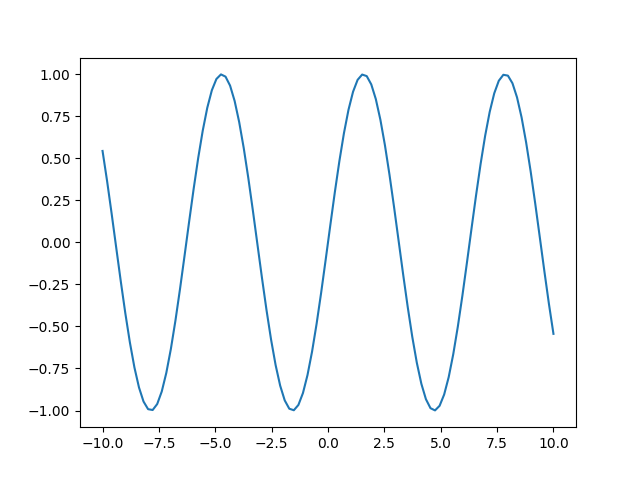
\includegraphics[width=0.8\textwidth]{images/basic.png}
\end{center}
\end{frame}

\subsection{Various plotting types}
\label{sec:orgd24ad66}

\begin{frame}[label={sec:orgf515c17}]{Different types of Plots}
\begin{center}
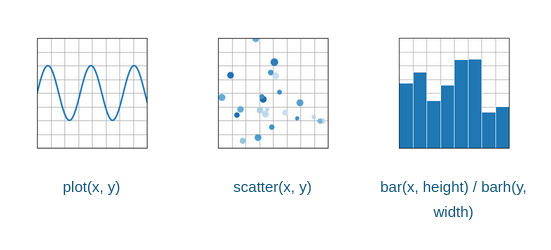
\includegraphics[width=0.6\textwidth]{images/plots.png}
\end{center}

There are many different types of plots that one can make using
matplotlib. These include the most popular:

\begin{itemize}
\item Line plots
\item Scatter plots
\item Bar plots
\item Histograms
\item Box plots
\item Image plots
\end{itemize}

We're going to take a look at how we create each type of plot, examining what
type of inputs they require.
\end{frame}

\begin{frame}[label={sec:org3b74388},fragile]{Line plots}
 We've already seen one example of a line plot. This plot draws a line between
each x,y point. For instance in the previous example, we created a sin wave by
'sampling' such wave using 100 samples from -10 to 10. Let's see what happens
when we sample only 10 points:

\begin{minted}[frame=lines,linenos=true,firstnumber=last,fontsize=\footnotesize,bgcolor=LightGray,xleftmargin=5pt,tabsize=2,breaklines=true,numbersep=10pt]{python}
x = np.linspace(-10, 10, 10)
y = np.sin(x)
plt.plot(x, y)
\end{minted}
\end{frame}

\begin{frame}[label={sec:org6896f81},fragile]{Line plots}
 We see the results are a less than ideal representation of a sin wave as \texttt{plot}
will simply draw a straight line from each point.

\begin{center}
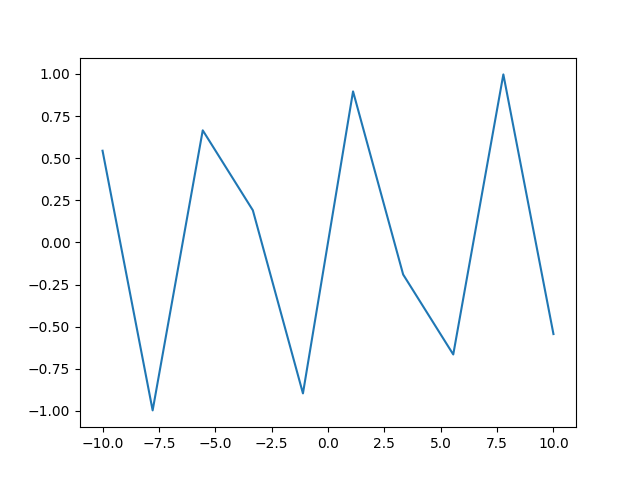
\includegraphics[width=0.6\textwidth]{images/lineplot.png}
\end{center}
\end{frame}

\begin{frame}[label={sec:orgc8cb70c},fragile]{Scatter plots}
 If we want to see where each sample of the sin wave is, we could use instead the
scatter plot, which will (by default) place a small circle at every x,y
value. To create a scatter plot, we use \texttt{scatter} instead of the \texttt{plot}
function. The arguments to this function are the same, however.

\begin{minted}[frame=lines,linenos=true,firstnumber=last,fontsize=\footnotesize,bgcolor=LightGray,xleftmargin=5pt,tabsize=2,breaklines=true,numbersep=10pt]{python}
x = np.linspace(-10, 10, 10)
y = np.sin(x)
plt.scatter(x, y)
\end{minted}
\end{frame}

\begin{frame}[label={sec:orgf69d301}]{Scatter plots}
Now we can see the position of each individual sample from the sin wave. If we,
once again, sample 100 points from this curve, we will see better results.

\begin{center}
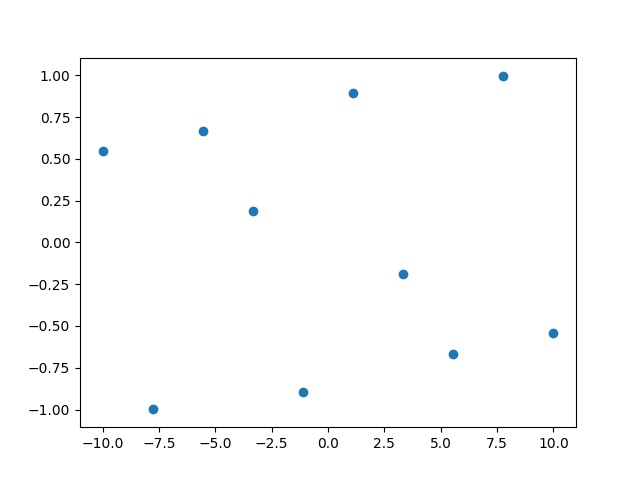
\includegraphics[width=0.5\textwidth]{images/scatter.png}
\end{center}
\end{frame}

\begin{frame}[label={sec:orgc74659e},fragile]{Scatter plots}
 \begin{minted}[frame=lines,linenos=true,firstnumber=last,fontsize=\footnotesize,bgcolor=LightGray,xleftmargin=5pt,tabsize=2,breaklines=true,numbersep=10pt]{python}
x = np.linspace(-10, 10, 100)
y = np.sin(x)
plt.scatter(x, y)
\end{minted}

\begin{center}
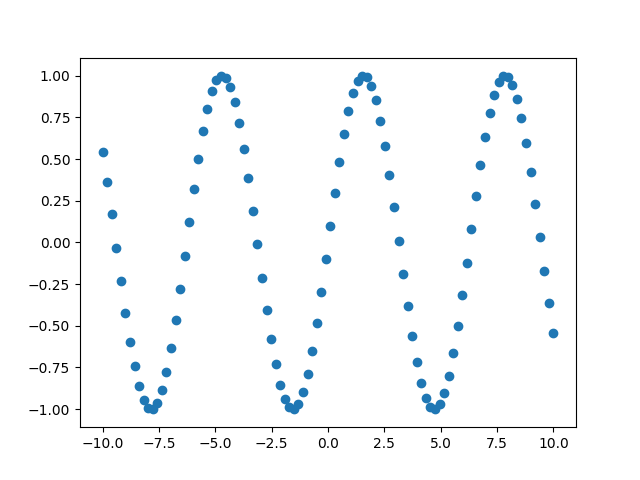
\includegraphics[width=0.5\textwidth]{images/scatter-2.png}
\end{center}
\end{frame}

\begin{frame}[label={sec:org9b81525},fragile]{Bar plots}
 Bar plots are a simple plot that again takes an \texttt{x} and a \texttt{y}, where x is the
numerical position of the bar's centre, and \texttt{y} is the height of the bar.

\begin{minted}[frame=lines,linenos=true,firstnumber=last,fontsize=\footnotesize,bgcolor=LightGray,xleftmargin=5pt,tabsize=2,breaklines=true,numbersep=10pt]{python}
x = np.arange(0, 8)
y = np.random.uniform(2, 7, len(x))
plt.bar(x, y)
\end{minted}

\begin{center}
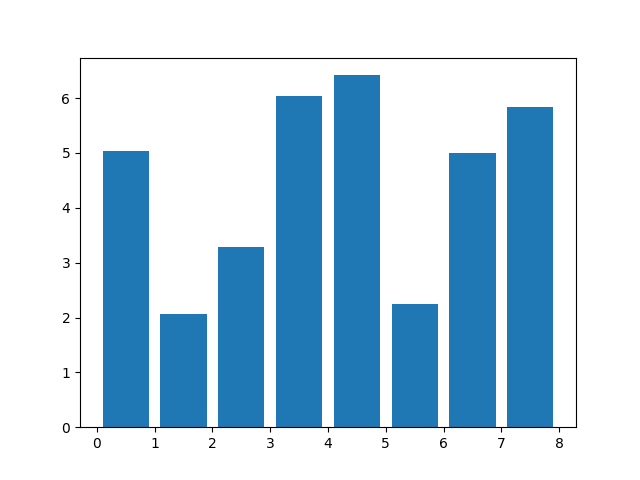
\includegraphics[width=0.5\textwidth]{images/bar.png}
\end{center}
\end{frame}

\begin{frame}[label={sec:org9e0ed9c},fragile]{Histograms}
 Histograms allow us to visualise the distribution of values. In matplotlib, we
can create a histogram of a vector by using the \texttt{hist} function that takes only
the vector as its argument.

\begin{minted}[frame=lines,linenos=true,firstnumber=last,fontsize=\footnotesize,bgcolor=LightGray,xleftmargin=5pt,tabsize=2,breaklines=true,numbersep=10pt]{python}
x = np.random.randn(1000)
plt.hist(x)
\end{minted}

\begin{center}
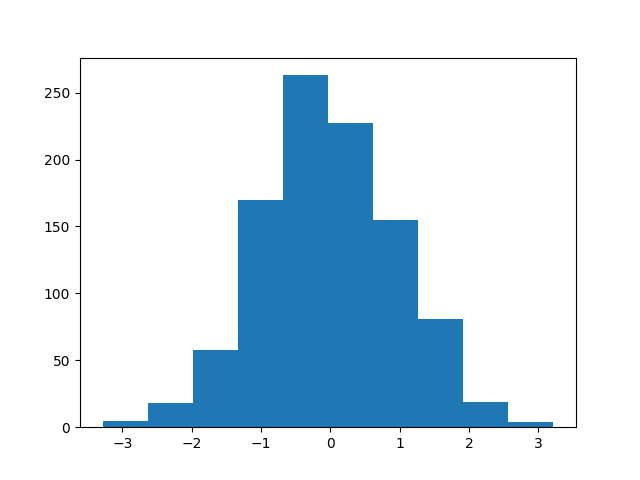
\includegraphics[width=0.5\textwidth]{images/hist.png}
\end{center}
\end{frame}

\begin{frame}[label={sec:org78c73e5},fragile]{Box plots}
 Box plots also allow us to visualise the distribution, but the distribution of
values within a group. In this example we're visualising the distribution of 3
groups. Using the \texttt{boxplot} function, we pass a matrix.

\begin{minted}[frame=lines,linenos=true,firstnumber=last,fontsize=\footnotesize,bgcolor=LightGray,xleftmargin=5pt,tabsize=2,breaklines=true,numbersep=10pt]{python}
x = np.random.randn(10, 3)
plt.boxplot(x)
\end{minted}

\begin{center}
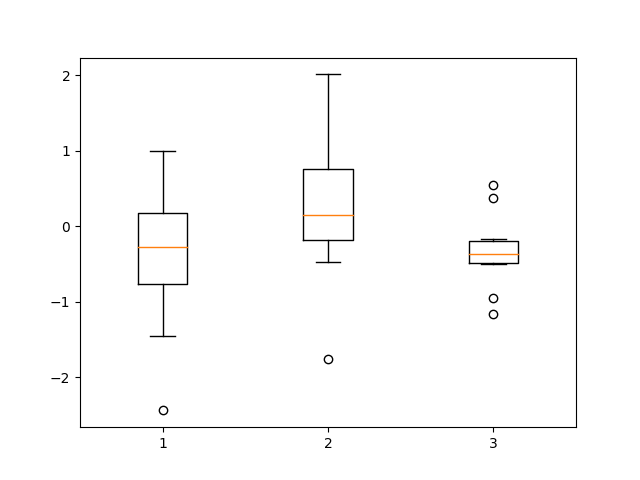
\includegraphics[width=0.5\textwidth]{images/boxplot.png}
\end{center}
\end{frame}

\begin{frame}[label={sec:org4abcf14},fragile]{Image plots}
 In matplotlib, we can plot an 'image' -- that is a 2D matrix -- using the \texttt{imshow}
function. For example:

\begin{minted}[frame=lines,linenos=true,firstnumber=last,fontsize=\footnotesize,bgcolor=LightGray,xleftmargin=5pt,tabsize=2,breaklines=true,numbersep=10pt]{python}
fig = plt.figure()
x = np.random.randn(10, 10)
plt.imshow(x)
\end{minted}

\begin{center}
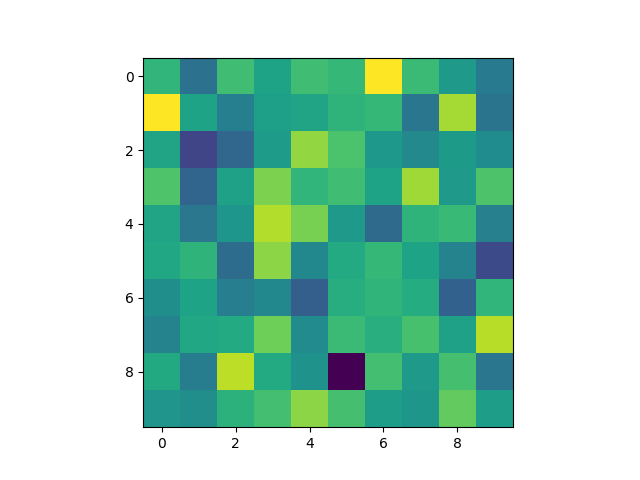
\includegraphics[width=0.5\textwidth]{images/imshow.png}
\end{center}
\end{frame}

\begin{frame}[label={sec:orgfa4b11d},fragile]{Image plots}
 Of course, given the name, we can then use \texttt{imshow} to plot an image as well, as
long as we have the image loaded as a 2D array of values.

\begin{minted}[frame=lines,linenos=true,firstnumber=last,fontsize=\footnotesize,bgcolor=LightGray,xleftmargin=5pt,tabsize=2,breaklines=true,numbersep=10pt]{python}
import PIL  # using the PIL module to read an image
img = np.array(PIL.Image.open("images/Lenna.png"))
plt.imshow(img)
\end{minted}

\begin{center}
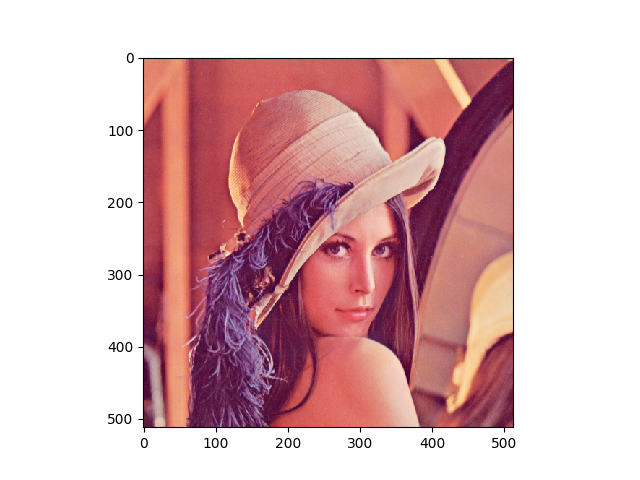
\includegraphics[width=0.5\textwidth]{images/imshow-2.png}
\end{center}
\end{frame}

\begin{frame}[label={sec:org5851345},fragile]{3 dimensional plots}
 3 dimensional plots require us to import another module from
matplotlib.

\begin{minted}[frame=lines,linenos=true,firstnumber=last,fontsize=\footnotesize,bgcolor=LightGray,xleftmargin=5pt,tabsize=2,breaklines=true,numbersep=10pt]{python}
from mpl_toolkits import mplot3d
\end{minted}

After importing this module, we can using the \emph{projection="3d"} and
carry on plotting as normal.

\begin{minted}[frame=lines,linenos=true,firstnumber=last,fontsize=\footnotesize,bgcolor=LightGray,xleftmargin=5pt,tabsize=2,breaklines=true,numbersep=10pt]{python}
fig = plt.figure()
ax = fig.gca(projection='3d')
theta = np.linspace(-4 * np.pi, 4 * np.pi, 100)
z = np.linspace(-2, 2, 100)
r = z**2 + 1
x = r * np.sin(theta)
y = r * np.cos(theta)
ax.plot(x, y, z, label='parametric curve')
ax.legend()
\end{minted}
\end{frame}

\begin{frame}[label={sec:orgffad524}]{3 dimensional plots}
\begin{center}
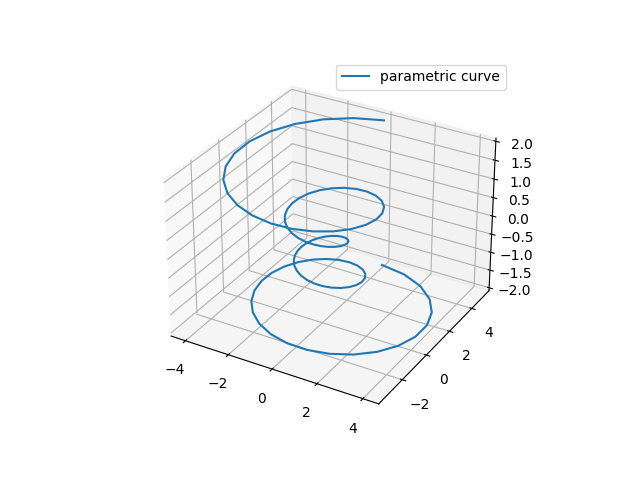
\includegraphics[width=0.8\textwidth]{images/3d-figure.png}
\end{center}
\end{frame}

\begin{frame}[label={sec:org9d7c78f}]{Different types of Plots}
There are many more different types of plots you can make using matplotlib. You
can find a comprehensive list at:

\url{https://matplotlib.org/stable/plot\_types/index.html}
\end{frame}

\subsection{Customising plots}
\label{sec:orgd358e71}

\begin{frame}[label={sec:org5966174},fragile]{Subplots}
 What if we wanted to create many plots side-by-side? For this we can use the
\texttt{subplots} function. This function takes the number of rows, and number of columns
to create. It returns two values, the first is the figure (entire figure), and
the second value is a list of sub figures. Using this list, we can place a plot
of each of them.

\begin{minted}[frame=lines,linenos=true,firstnumber=last,fontsize=\footnotesize,bgcolor=LightGray,xleftmargin=5pt,tabsize=2,breaklines=true,numbersep=10pt]{python}
x = np.linspace(-10, 10, 100)
y = np.sin(x)
z = np.cos(y)

fig, ax = plt.subplots(1, 2)
# ax is a list of sub figures
ax[0].plot(x, y)
ax[1].plot(x, z)
\end{minted}
\end{frame}

\begin{frame}[label={sec:orgd7910c0}]{Subplots}
\begin{center}
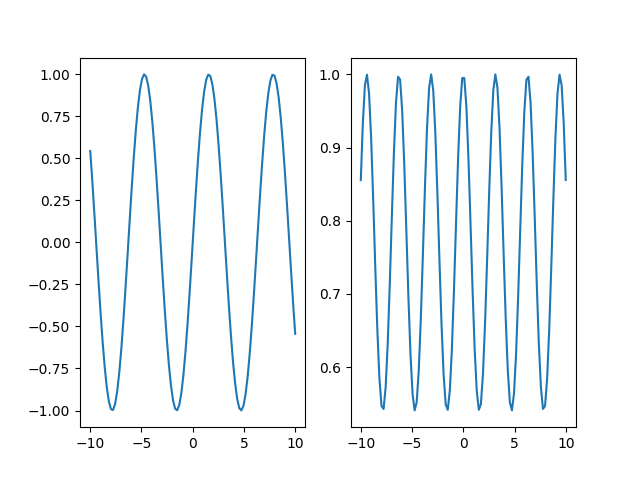
\includegraphics[width=0.6\textwidth]{images/subplots.png}
\end{center}
\end{frame}

\begin{frame}[label={sec:org1e6a12f},fragile]{Adding a legend}
 Or we could put them onto the same plot. Matplotlib will automatically give them
a different colour. If we use the \texttt{label} argument to \texttt{plot}, we can also give them
a name that will appear when we call \texttt{legend()}.

\begin{minted}[frame=lines,linenos=true,firstnumber=last,fontsize=\footnotesize,bgcolor=LightGray,xleftmargin=5pt,tabsize=2,breaklines=true,numbersep=10pt]{python}
x = np.linspace(-10, 10, 100)
y = np.sin(x)
z = np.tan(y)
fig, ax = plt.subplots()
ax.plot(x, y, label="sin(x)")
ax.plot(x, z, label="tan(x)")
ax.legend()
\end{minted}
\end{frame}

\begin{frame}[label={sec:org353839f}]{Adding a legend}
\begin{center}
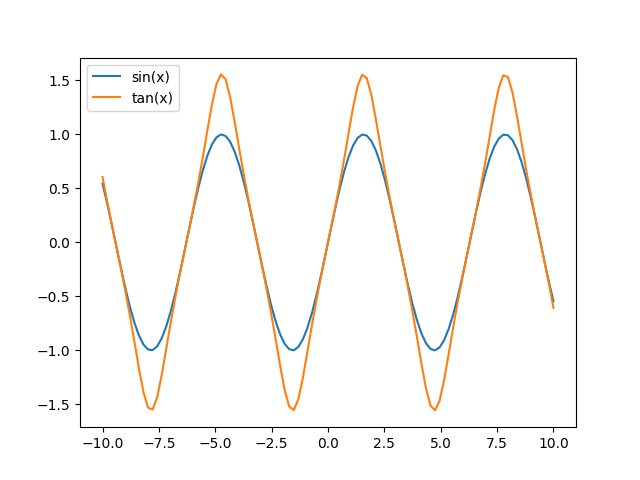
\includegraphics[width=0.7\textwidth]{images/legend.png}
\end{center}
\end{frame}

\begin{frame}[label={sec:orge68331d},fragile]{Position the legend in different places}
 We can change the position of the legend by specifying a different integer value
for the \texttt{loc} argument (or string values such as 'upper left', 'upper right',
\ldots{}). Additionally, we can change the number of columns the legend has with the
\texttt{ncol} argument.

\begin{minted}[frame=lines,linenos=true,firstnumber=last,fontsize=\footnotesize,bgcolor=LightGray,xleftmargin=5pt,tabsize=2,breaklines=true,numbersep=10pt]{python}
x = np.linspace(-10, 10, 100)
y = np.sin(x)
z = np.tan(y)

fig, ax = plt.subplots()
ax.plot(x, y, label="sin(x)")
ax.plot(x, z, label="tan(x)")
ax.legend(loc=1, ncol=2)
\end{minted}

You can find the API reference for the different arguments to legend at: \url{https://matplotlib.org/stable/api/legend\_api.html?highlight=legend\#module-matplotlib.legend}
\end{frame}

\begin{frame}[label={sec:org772edff}]{Position the legend in different places}
\begin{center}
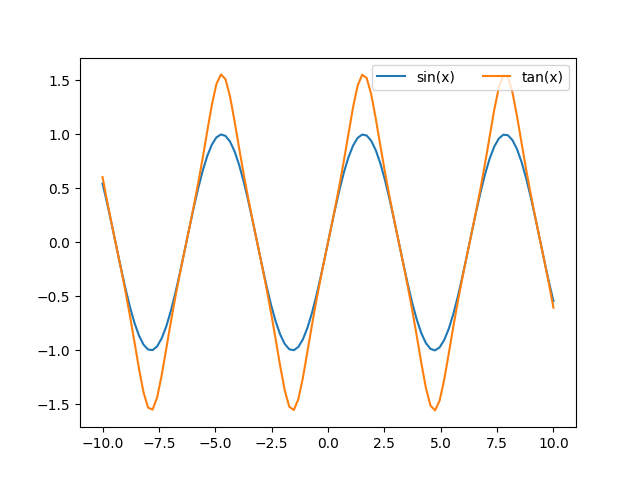
\includegraphics[width=0.8\textwidth]{images/legend-2.png}
\end{center}
\end{frame}

\begin{frame}[label={sec:orgb81f857},fragile]{Modifying the x/y axis}
 Good graphs always have their axis's labelled. To do this in matplotlib, if we
have a subplot object, we use \texttt{set\_xlabel}, or we can use \texttt{plt.xlabel(...)}. Here is
an example with an subplot object:

\begin{minted}[frame=lines,linenos=true,firstnumber=last,fontsize=\footnotesize,bgcolor=LightGray,xleftmargin=5pt,tabsize=2,breaklines=true,numbersep=10pt]{python}
x = np.linspace(-10, 10, 100)
y = np.sin(x)
z = np.tan(y)

fig, ax = plt.subplots()
ax.plot(x, y, label="sin(x)")
ax.plot(x, z, label="tan(x)")
ax.legend(loc=1, ncol=2)
ax.set_xlabel("x")
ax.set_ylabel("y")
\end{minted}
\end{frame}

\begin{frame}[label={sec:org2961c67}]{Modifying the x/y axis}
\begin{center}
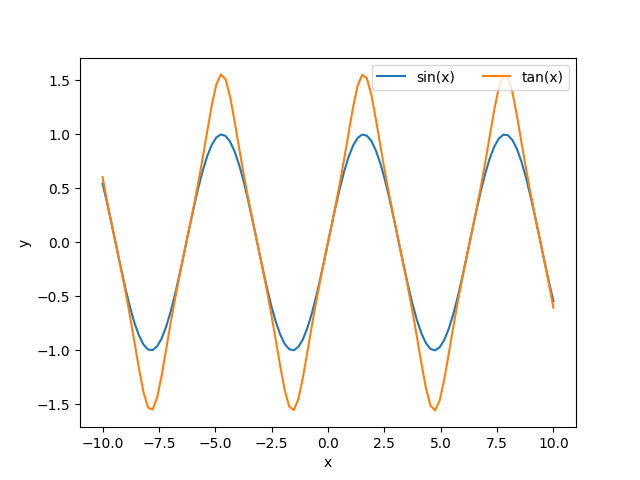
\includegraphics[width=0.8\textwidth]{images/axis.png}
\end{center}
\end{frame}

\begin{frame}[label={sec:org89bd78b},fragile]{Changing figure size}
 A common change you may want to make to your figure is to change its size or
aspect ratio. \texttt{figure()} or \texttt{subplots()} take an optional argument called
\texttt{figsize}. This argument expects a tuple representing the width and height of the
figure in inches.

\begin{minted}[frame=lines,linenos=true,firstnumber=last,fontsize=\footnotesize,bgcolor=LightGray,xleftmargin=5pt,tabsize=2,breaklines=true,numbersep=10pt]{python}
fig = plt.figure(figsize=(8, 2.5))

# or most likely
fig, ax = plt.subplots(figsize=(8, 2.5))
x = np.linspace(-10, 10, 100)
y = np.sin(x)
z = np.tan(y)
ax.plot(x, y, label="sin(x)")
ax.plot(x, z, label="tan(x)")
ax.legend(loc=1, ncol=2)
ax.set_xlabel("x")
ax.set_ylabel("y")
\end{minted}

Here we are creating a figure with 8 inches of width, and 2.5 inches of height.
\end{frame}

\begin{frame}[label={sec:org09712eb}]{Changing figure size}
\begin{center}
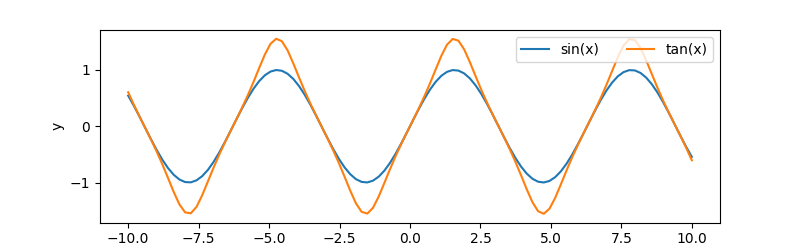
\includegraphics[width=.9\linewidth]{images/fig-size.png}
\end{center}
\end{frame}

\begin{frame}[label={sec:orgc9d57e6},fragile]{Changing figure size}
 This is especially useful when you have many sub-figures, as by default, they
will be 'squashed' into the default aspect ratio. We can 'give them more space'
by modifying this \texttt{figsize} argument when creating the many sub-figures.

\begin{minted}[frame=lines,linenos=true,firstnumber=last,fontsize=\footnotesize,bgcolor=LightGray,xleftmargin=5pt,tabsize=2,breaklines=true,numbersep=10pt]{python}
fig, ax = plt.subplots(1, 2, figsize=(8, 2.5))
x = np.linspace(-10, 10, 100)
y = np.sin(x)
z = np.tan(y)
ax[0].plot(x, y, label="sin(x)")
ax[1].plot(x, z, label="tan(x)")
\end{minted}
\end{frame}

\begin{frame}[label={sec:org76d12fd}]{Changing figure size}
\begin{center}
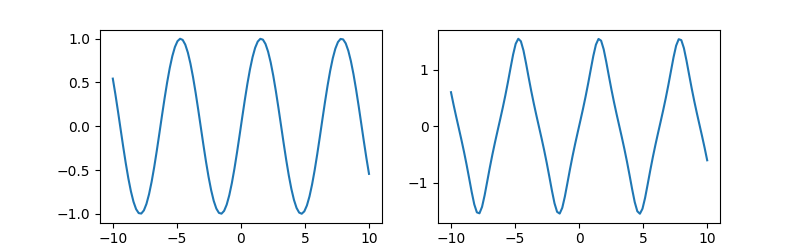
\includegraphics[width=0.9\textwidth]{images/figsize-2.png}
\end{center}
\end{frame}

\begin{frame}[label={sec:orgd5a73c2}]{Line properties}
When creating a plot, there are many different properties you can change. Some
of these include:

\begin{itemize}
\item color -- the colour of the line
\item alpha -- the amount of transparency (1.0 is opaque, 0.0 is transparent)
\item linewidth, lw -- the width of the stroke width
\item linestyle, ls -- the style of the line (i.e. a dotted line)
\end{itemize}

There are also some properties for the markers, i.e. the circles in the scatter
plot. These properties are:

\begin{itemize}
\item marker -- the type of marker (you can use different shapes instead of a circle
\item markersize -- the size of the mark
\item markerfacecolor -- colour of the marker
\item markeredgewidth -- outline width of the marker.
\end{itemize}
\end{frame}

\begin{frame}[label={sec:orga728e6d},fragile]{Line properties}
 If this example we are modifying some of the line properties that include the
color (c), setting it to a string value of "green". The linewidth (lw) to be
thicker, and making the line to be a dotted line by specifying the linestyle
(ls) to "=--=\{".

\begin{minted}[frame=lines,linenos=true,firstnumber=last,fontsize=\footnotesize,bgcolor=LightGray,xleftmargin=5pt,tabsize=2,breaklines=true,numbersep=10pt]{python}
fig = plt.figure()
x = np.linspace(-5, 5, 100)
y = np.sin(x)
plt.plot(x, y,
         c="green", # or color
         lw=3, # or linewidth
         ls="--")
\end{minted}

\begin{center}
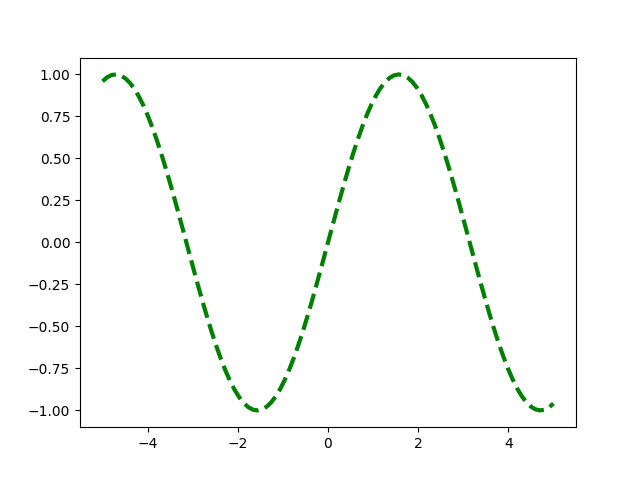
\includegraphics[width=0.4\textwidth]{images/linestyles.png}
\end{center}
\end{frame}

\begin{frame}[label={sec:org4e48afd},fragile]{Colormaps}
 When we create a heatmap using \texttt{imshow}, the gradients of colour are automatically
set. Yet, we can control the colour gradient using a colour map. First we must
import \texttt{cm} from matplotlib:

\begin{minted}[frame=lines,linenos=true,firstnumber=last,fontsize=\footnotesize,bgcolor=LightGray,xleftmargin=5pt,tabsize=2,breaklines=true,numbersep=10pt]{python}
from matplotlib import cm
\end{minted}

Then we can get a colour map with 10 levels using \texttt{get\_cmap}:

\begin{minted}[frame=lines,linenos=true,firstnumber=last,fontsize=\footnotesize,bgcolor=LightGray,xleftmargin=5pt,tabsize=2,breaklines=true,numbersep=10pt]{python}
blues = cm.get_cmap("Blues", 10) # 10 levels
reds = cm.get_cmap("Reds", 2) # 2 levels
\end{minted}

You can find a full list of different colour maps at: \url{https://matplotlib.org/stable/tutorials/colors/colormaps.html}
\end{frame}

\begin{frame}[label={sec:orgf4397ee},fragile]{Colourmaps}
 Now that we have our new colour maps, we can pass it as an \texttt{cmap} argument when we
create a plot.

\begin{minted}[frame=lines,linenos=true,firstnumber=last,fontsize=\footnotesize,bgcolor=LightGray,xleftmargin=5pt,tabsize=2,breaklines=true,numbersep=10pt]{python}
x = np.random.randn(10, 10)
y = np.random.randn(10, 10)
fig, ax = plt.subplots(1, 2, figsize=(8, 3))
p1 = ax[0].imshow(x, cmap=blues)
p2 = ax[1].imshow(y, cmap=reds)
fig.colorbar(p1, ax=ax[0])
fig.colorbar(p2, ax=ax[1])
\end{minted}

\begin{center}
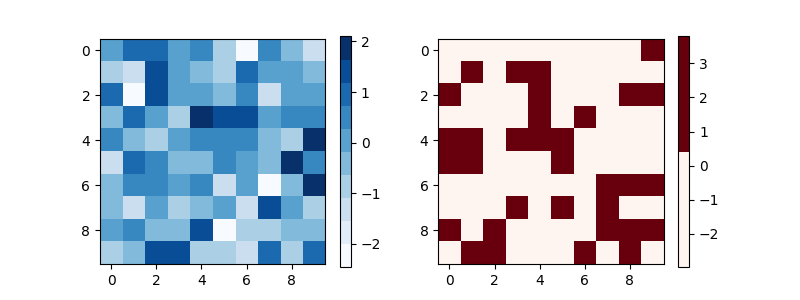
\includegraphics[width=0.8\textwidth]{images/colourmaps.png}
\end{center}
\end{frame}

\begin{frame}[label={sec:org4843eda},fragile]{Ticks}
 If we want to customise the numbers along each axis, we use the \texttt{set\_xticks} for
the x-axis and \texttt{set\_yticks} for the y-axis. These functions take the list of
locations for each 'tick', and optionally a list of labels to use instead of the numbers.

\begin{minted}[frame=lines,linenos=true,firstnumber=last,fontsize=\footnotesize,bgcolor=LightGray,xleftmargin=5pt,tabsize=2,breaklines=true,numbersep=10pt]{python}
x = np.linspace(-2, 2, 100)
y = np.sin(x)

bx = np.arange(2, 7)
by = np.random.uniform(2, 7, len(bx))

fig, ax = plt.subplots(1, 2, figsize=(8, 3))
ax[0].plot(x, y)
ax[0].set_xticks([-2, 0, 2])
ax[1].bar(bx, by)
ax[1].set_xticks(bx, ["a", "b", "c", "d", "e"])
\end{minted}
\end{frame}

\begin{frame}[label={sec:org9bdf587}]{Ticks}
\begin{center}
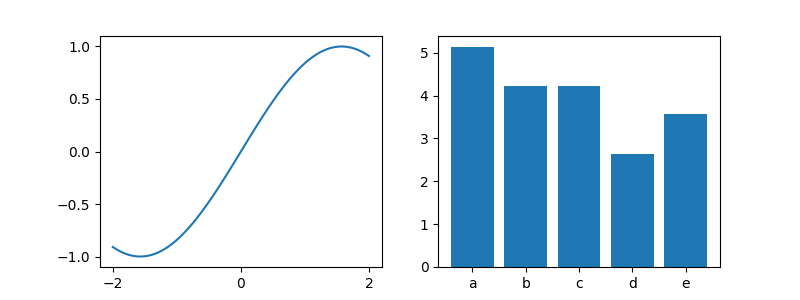
\includegraphics[width=0.9\textwidth]{images/ticks.png}
\end{center}
\end{frame}

\begin{frame}[label={sec:orgef51df6},fragile]{Grids}
 In all of the previous plots, the background has no grids, they are simply
white. If we wanted to add grid lines to the plot we use the \texttt{.grid()}
method. This function, by default, adds the major grid lines.

\begin{minted}[frame=lines,linenos=true,firstnumber=last,fontsize=\footnotesize,bgcolor=LightGray,xleftmargin=5pt,tabsize=2,breaklines=true,numbersep=10pt]{python}
x = np.linspace(-2, 2, 100)
y = np.sin(x)
z = np.tan(x)
fig, ax = plt.subplots(1, 2, figsize=(8, 3))
ax[0].plot(x, y)
ax[0].grid()
ax[1].plot(x, z)
ax[1].grid(which="both", color="r")
\end{minted}
\end{frame}

\begin{frame}[label={sec:org68e39ca}]{Grids}
\begin{center}
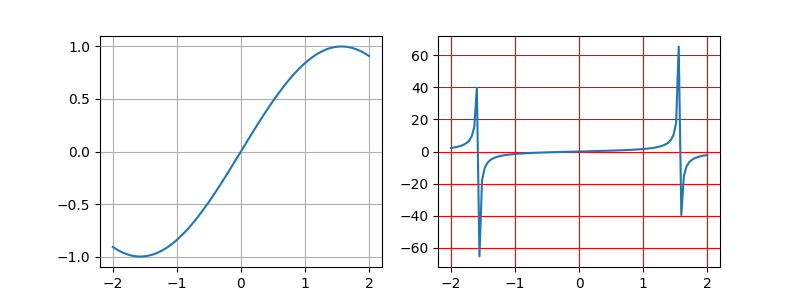
\includegraphics[width=0.9\textwidth]{images/grids.png}
\end{center}
\end{frame}

\begin{frame}[label={sec:orga3bf2d5},fragile]{Scale}
 The default behaviour of matplotlib is to plot using a linear scale. In certain
situations, we want view the plot using a different scale. For this we can use \texttt{set\_yscale}.

\begin{minted}[frame=lines,linenos=true,firstnumber=last,fontsize=\footnotesize,bgcolor=LightGray,xleftmargin=5pt,tabsize=2,breaklines=true,numbersep=10pt]{python}
x = np.linspace(-2, 10, 100)
y = np.exp(x)
fig, ax = plt.subplots(1, 2, figsize=(8, 3))
ax[0].plot(x, y)
ax[0].grid()
ax[1].plot(x, y)
ax[1].set_yscale('log')
ax[1].grid()
\end{minted}

\begin{center}
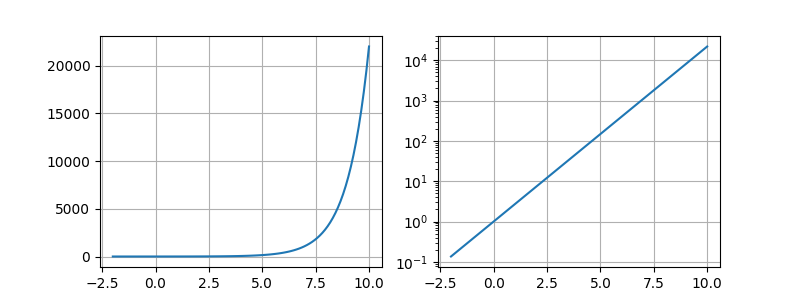
\includegraphics[width=0.8\textwidth]{images/scale.png}
\end{center}
\end{frame}

\begin{frame}[label={sec:orgddd9490},fragile]{Setting the plot limits}
 By default, matplotlib will calculate the minimum and maximum values of the
data, and use those values to set the limits of the plot. Using \texttt{set\_xlim} and
\texttt{set\_ylim} we can change this default behaviour.

\begin{minted}[frame=lines,linenos=true,firstnumber=last,fontsize=\footnotesize,bgcolor=LightGray,xleftmargin=5pt,tabsize=2,breaklines=true,numbersep=10pt]{python}
x = np.linspace(-2, 2, 100)
y = np.sin(x)
fig, ax = plt.subplots(1, 2, figsize=(8,3))
ax[0].plot(x, y)
ax[0].set_ylim(-1, 2)
ax[1].plot(x, y)
ax[1].set_xlim(-3, 3)
\end{minted}

\begin{center}
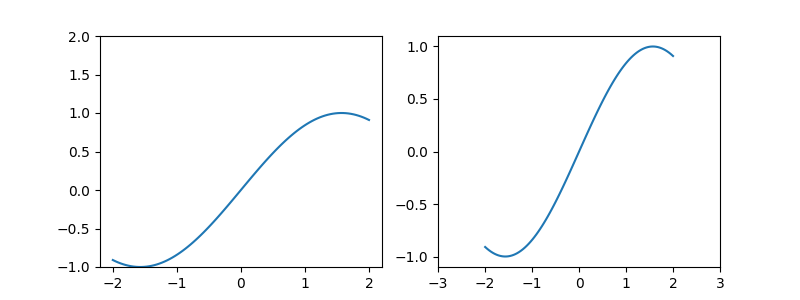
\includegraphics[width=0.7\textwidth]{images/limits.png}
\end{center}
\end{frame}

\begin{frame}[label={sec:org91d9a11},fragile]{Annotations}
 We can annotate our plot in a number of way:
\begin{itemize}
\item .axhline -- plot a horizontal line (axvline for vertical lines)/
\item .annotate -- add text to the plot at a certain position.
\end{itemize}

\begin{minted}[frame=lines,linenos=true,firstnumber=last,fontsize=\footnotesize,bgcolor=LightGray,xleftmargin=5pt,tabsize=2,breaklines=true,numbersep=10pt]{python}
x = np.linspace(-2, 2, 100)
y = np.sin(x)
fig, ax = plt.subplots()
ax.plot(x, y)
ax.axhline(0, c='gray', ls='--')
ax.annotate("0th line", (-2, 0), xytext=(-1.5, 0.25),
            arrowprops=dict(facecolor='black', shrink=0.05,
                            width=0.5, headwidth=5.0))
\end{minted}
\end{frame}

\begin{frame}[label={sec:org299f881}]{Annotations}
\begin{center}
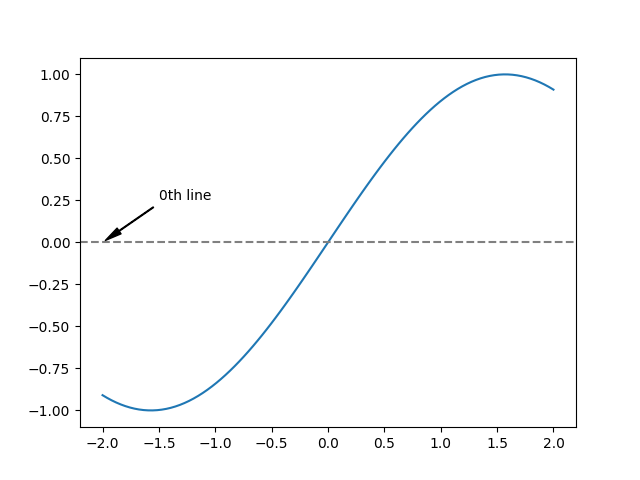
\includegraphics[width=0.8\textwidth]{images/annotations.png}
\end{center}
\end{frame}

\begin{frame}[label={sec:org791cf80},fragile]{Creating a twin axes plot}
 Sometimes you will want to display multiple sub-plots on the same plot, but
where each have a very different range in values. Instead of having a single
y-axis, with \texttt{twinx()} we can create a two y-axis plot.

\begin{minted}[frame=lines,linenos=true,firstnumber=last,fontsize=\footnotesize,bgcolor=LightGray,xleftmargin=5pt,tabsize=2,breaklines=true,numbersep=10pt]{python}
x = np.arange(10, 100)
y = np.exp(x)
z = np.log(x)

fig, ax = plt.subplots(1, 2)
ax[0].plot(x, y, label="exp(x)")
ax[0].plot(x, z, label="log(x)")
ax[0].legend()

ax2 = ax[1].twinx()
ax[1].plot(x, y)
ax2.plot(x, z, color="orange")
ax2.tick_params(axis="y", labelcolor="orange")
\end{minted}
\end{frame}

\begin{frame}[label={sec:org41dadcd}]{Creating a twin axes plot}
\begin{center}
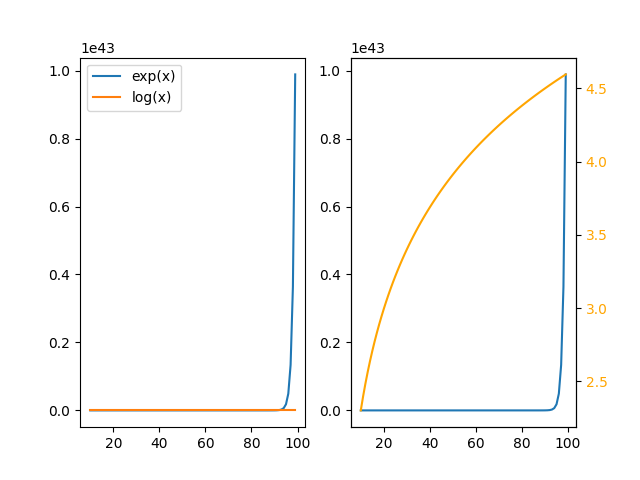
\includegraphics[width=0.8\textwidth]{images/twinx.png}
\end{center}
\end{frame}

\begin{frame}[label={sec:orge55807f}]{Learn more}
There are many many more types of plots you can create with matplotlib. I would
recommend that you read the documentation to fully appreciate everything that it
can visualise:

\begin{itemize}
\item Gallery -- \url{https://matplotlib.org/stable/gallery/index.html}
\item Plotting tutorials -- \url{https://matplotlib.org/stable/tutorials/index.html}
\item Basic plot types -- \url{https://matplotlib.org/stable/plot\_types/index.html}
\end{itemize}
\end{frame}
\end{document}
